\scanpage{19}
Dém. par récurrence, c'est trivial si $\operatorname{card} I=0,1$ Le cas $\operatorname{card} I=2$ a été vu. Cas général \unsure{avec} $\operatorname{card} I\geqslant 3$, on choisit $J$ comme dessus. Il suffit de voir que les ens.
% G01: complete first U, including its three entrance/body paths.
% Shape candidates: U with entrance return | cancelled equality before U.
% Source origin (580,535); x right, y down; one local unit is one source pixel.
% The local rectangle is [0,0,120,70]; baseline y=60; scale 0.008 cm/unit.
\figure{\[
\mathord{\unsure{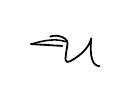
\begin{tikzpicture}[x=0.008cm,y=-0.008cm,baseline=(u-base),line cap=round,line join=round]
\coordinate (u-base) at (0,60);
\path[use as bounding box] (0,0) rectangle (120,70);
\draw[line width=.65pt] (36,14) .. controls (50,10) and (66,17) .. (63,28) .. controls (59,53) and (58,57) .. (68,53) .. controls (90,41) and (98,28) .. (101,17) .. controls (98,46) and (103,61) .. (114,61);
\draw[line width=.55pt] (6,26) .. controls (20,22) and (41,16) .. (60,22);
\draw[line width=.65pt] (5,26) -- (55,29);
\end{tikzpicture}}}_{J,i}\cap\Sigma_i^+,\ U_{J,i}\cap\Sigma_i^-
\]}
ont la forme précédente, il suffit de le voir pour \(\underset{\phantom{\text{l'un}}\unsure{\cdot}}{\text{\unsure{l'une|l'un}}}\) des deux.
% G02: one visible point below the terminal run of l'une/l'un; attachment unresolved.

Par hyp. de récurrence, \unsure{on a}
% G03: first footed union, with its rounded inner return and upright retraces.
% Glyph candidates coprod | bigsqcup remain unresolved (original C row R03).
% Source origin (895,965); local rectangle [0,0,125,90]; baseline y=80.
\figure{\[
U_{J,i}=X\setminus\mathop{\unsure{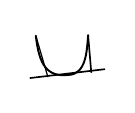
\begin{tikzpicture}[x=0.008cm,y=-0.008cm,baseline=(union-one-base),line cap=round,line join=round]
\coordinate (union-one-base) at (0,80);
\path[use as bounding box] (0,0) rectangle (125,90);
\draw[line width=.7pt] (13,13) .. controls (18,58) and (30,79) .. (65,75) .. controls (93,74) and (94,37) .. (96,12);
\draw[line width=.6pt] (4,80) -- (122,66);
\draw[line width=.45pt] (13,13) -- (32,78);
\draw[line width=.6pt] (96,12) -- (101,71);
\end{tikzpicture}}}\limits_{\alpha\in \deleted{\unsure{J|j}}K_0}\widehat{\Sigma}_\alpha^+
\]}
où
\[
\left\{\begin{aligned}
&\deleted{\Sigma_{\unsure{\alpha|0}}}K_0\subset J\\
&\Sigma_\alpha^+\in\pi_0(X\setminus E_\alpha)\qquad (\forall\,\alpha\in K_0)\\
&\widehat{\Sigma}_\alpha^+=\Sigma_\alpha^+\cup E_\alpha.
\end{aligned}\right.
\]
\unsure{On a|\deleted{On}On a} donc
% G04: second footed union, inspected independently in half b.
% Same glyph candidates as G03; the first-occurrence uncertainty is printed at G03.
% Source origin (820,1605); local rectangle [0,0,95,93]; baseline y=80.
\figure{\[
U=U_{J,i}\cap\Sigma_i^-=X\setminus\left(\mathop{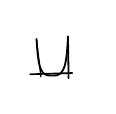
\begin{tikzpicture}[x=0.008cm,y=-0.008cm,baseline=(union-two-base),line cap=round,line join=round]
\coordinate (union-two-base) at (0,80);
\path[use as bounding box] (0,0) rectangle (95,93);
\draw[line width=.65pt] (14,18) .. controls (17,65) and (20,78) .. (40,76) .. controls (61,79) and (62,49) .. (64,14);
\draw[line width=.6pt] (4,74) -- (71,72);
\draw[line width=.45pt] (14,18) -- (21,78);
\draw[line width=.65pt] (64,14) -- (65,80);
\end{tikzpicture}}\limits_{\alpha\in K_0}\widehat{\Sigma}_\alpha^+\ \cup\ \widehat{\Sigma}_i^+\right)
\]}
\deleted{Soit} Au \unsure{dernier|deuxième} $=$, dans la \deleted{\unsure{somme|réunion}} réunion $\bigcup_{\alpha\in K_0}\widehat{\Sigma}_\alpha^+$, il suffit de se borner \unsure{à|:} sommer sur les \deleted{$\Sigma$} $\alpha\in K_0$ tels que $\widehat{\Sigma}_\alpha^+\not\subset\widehat{\Sigma}_i^+$ i.e. $\Sigma_\alpha^+\not\subset\Sigma_i^+$ soit $K_1$ cet ens., donc
\[
U=X\setminus\left(\bigcup_{\alpha\in K_1}\widehat{\Sigma}_\alpha^+\ \cup\ \widehat{\Sigma}_i^+\right)
\]
% archive sheet number: 18
